
\documentclass[12pt]{article}

\usepackage[T1]{fontenc}
\usepackage[utf8]{inputenc}
\usepackage[pdftex]{graphicx}
\usepackage{float}
\usepackage{graphics}
%\usepackage{natbib}
\usepackage{amsmath}
\usepackage{siunitx}
\usepackage{epstopdf}
\usepackage[english]{babel}
\usepackage{lmodern}
\usepackage{isotope}
\usepackage{listings}
\usepackage{chngcntr}
\usepackage{subcaption}
%\usepackage[square,numbers]{natbib}
%\bibliographystyle{ksfh_nat}

\counterwithin{figure}{section}
\def\thickhrulefill{\leavevmode \leaders \hrule height 1pt\hfill \kern \z@}

\usepackage{hyperref}
\usepackage{color}
\definecolor{codegreen}{rgb}{0,0.6,0}
\definecolor{codegray}{rgb}{0.5,0.5,0.5}
\definecolor{codepurple}{rgb}{0.58,0,0.82}
\definecolor{backcolour}{rgb}{0.95,0.95,0.92}

\lstdefinestyle{mystyle}{
	backgroundcolor=\color{backcolour},   
	commentstyle=\color{codegreen},
	keywordstyle=\color{magenta},
	numberstyle=\tiny\color{codegray},
	stringstyle=\color{codepurple},
	basicstyle=\footnotesize,
	breakatwhitespace=false,         
	breaklines=true,                 
	captionpos=b,                    
	keepspaces=true,                 
	numbers=left,                    
	numbersep=5pt,                  
	showspaces=false,                
	showstringspaces=false,
	showtabs=false,                  
	tabsize=2
}

\lstset{style=mystyle}
\begin{document}

\begin{figure}
\begin{minipage}{0.5\linewidth}
\begin{flushleft}
\includegraphics[width=5cm]{pics/ethlogo_black.eps}
\end{flushleft}
\end{minipage}
\hspace{0.05cm}
\begin{minipage}{0.5\linewidth}
\begin{flushright}
Manual number:\hspace{2cm}\\[0.5cm]
\includegraphics[width=4cm]{pics/VP-Logo.eps}
\end{flushright}
\end{minipage}
\hrule height 1pt\hfill \\[3cm]
\end{figure} 

\title{Drift Chamber\\ Instructions}
\author{D. Hits, G. Guyer, M. Setz}
\date{rev. D. Hits, \today}
\maketitle

\newpage
\section{Introduction}

This manual contains only a brief introduction to the processes occurring in a drift chamber. In order to gain a more complete understanding of the physics of drift chambers the references at the end of this manual should be consulted \cite{DriftChamberBook, knoll, NIMwiki}. 

Drift chambers belong to the most important measurement devices of nuclear and particle physics. They are a central aspect of nearly every large experiment in high energy physics. In this experiment a small drift chamber is operated and characterized, in order to reconstruct the trajectories of particles originating from cosmic radiation. 

If a charged particle travels through a gas volume it leaves a trail of ionized gas atoms and free electrons behind. By applying an electric field the ions and electrons can be separated, which generates an electric signal. This signal, however, is very small. A high-energy particle with an elementary charge produces only about 100 electron/ion-pairs by going through one centimeter of air. Single particles are therefore only detectable after amplifying this signal. 

In a detector filled with gas there is a simple way to amplify the signal inside the detector, even before it is measured on the outside. If the electric field is sufficiently strong, the free electrons can be accelerated to energies large enough to ionize gas atoms and create an avalanche which will result in an electric signal many times higher than the original one. The required electric field strengths are easily generated around very thin wires. By using very thin signal wires, one can therefore easily create a detectable signal. Hence already a simple structure allows the detection of particle radiation. Many detectors are based on this principle, from a simple Geiger counter up to time projection chambers in high energy experiments with several thousand wires. 

A drift chamber additionally makes use of the fact that the amplification of the signal only occurs when the free electrons reach the region of strong fields in the immediate proximity of a wire. Before reaching this point the electrons simply drift along the electric field lines, without increasing their numbers. With a known drift velocity and a measured time difference between the arrival of the particle and the detection of the electric signal, the distance between the signal wire and the trajectory of the particle can therefore be calculated. The location can be reconstructed in such a chamber with a resolution to a fraction of a millimeter. By combining the position measurement of multiple wires, the trajectory of the particle can be reconstructed. Figure~\ref{fig:structure} shows the general structure of a drift chamber. It is described in more detail in section~\ref{measurementsetupdriftchamber}.


Figure~\ref{fig:H1_detector} shows traces of particles, which were being generated by a electron-proton-collision in the H1-Detector at the HERA storage ring. The paths are curved, because the detector is inside a strong magnetic field. The curvature is a measure of the charge and momentum of the particles. By the way the gas inside the H1-Detector is identical to the gas used in our experiment. 

\begin{figure}[h]
\includegraphics[width=13cm]{pics/PRINZIP}
\centering
\caption{General structure of a drift chamber.}
\label{fig:structure}
\end{figure}

\newpage

\begin{figure}[!h]
\includegraphics[width=13cm]{pics/H1-eps-converted-to.pdf}
\centering
\caption{Particle trajectories in the central drift chamber of the H1 experiment. The drift chamber is cylindrical and the anode wires are parallel to the cylindrical axis, therefore they are perpendicular to the image plane. Each point represents a wire which detected a signal. The positions are corrected by means of drift duration.}
\label{fig:H1_detector}
\end{figure}

\section{Electron drift}

The electrons released by ionization get quickly to thermal equilibrium through elastic collisions with the gas atoms. The electrons then move in arbitrary, frequently changing directions. Therefore we can assume that the average kinetic energy is like in an ideal gas
\begin{equation}
< \frac{1}{2} m v^2 > = \frac{3}{2} k T.
\end{equation}
At room temperature this correlates to a velocity of \SI{120}{\kilo\meter\per\second}!

Between the collisions the electrons get accelerated by the electric field. Thus on a macroscopic scale we can say that the electrons move in the direction of the electric field lines.   

For a start we look at a group of electrons all traveling with velocity $v$. Along a way $dx$ a fraction $N \sigma dx$ of the electrons collide with a gas atom, where $N$ is the number of gas atoms per unit volume and $\sigma$ the total collision cross section. Let $n(t)$ be the number of electrons which did not collide with a gas atom in a time $t$ since the last collision. Thus $n(t)$ can be calculated using
\begin{equation}
dn(t) = - N \sigma v dt = -\frac{v}{l} dt.
\label{eq:dn(t)}
\end{equation}

The quantity $l \equiv N \sigma$ is called the mean free path of the electrons in the gas. Integrating (\ref{eq:dn(t)}) yields
\begin{equation}
n(t) = n_0 \exp\Big(-\frac{v}{l} t \Big).
\end{equation}

An electron experiences a constant force $e \vec{E}$ on the path between two collisions. Therefore additionally to the free movement the electron covers the distance 
\begin{equation}
\Delta s = \frac{1}{2} \frac{eE}{m} \Delta t^2
\end{equation}
along the $\vec{E}$-field.

The mean drift velocity for electrons with velocity $v$ is thus
\begin{align*}
 v_D(v) & = \frac{\int \Delta s(t) e^{-\frac{v}{l} t}dt}{\int t e^{-\frac{v}{l}}dt} \\
 & = \frac{1}{2}\frac{eE}{m} \frac{\int t^2 e^{-\frac{v}{l} t}dt}{\int t e^{-\frac{v}{l}}dt} = \frac{eE}{m} \frac{l}{v}.
\end{align*}

In reality not all electrons are moving with the same velocity. Instead the velocities are distributed as a Maxwell-Boltzmann distribution. Thus to get the mean drift velocity for the whole electron cloud, one has to average over the thermal velocities. The drift velocity of the electron cloud is therefore
\begin{equation} \label{eq:simple_drift}
v_D = \frac{eE}{m} < \frac{l}{v} > = \frac{eE}{m} \tau,
\end{equation}
where $\tau$ is the mean time between two collisions of an electron with a gas atom.

According to this simple calculation one expects the drift velocity to increase proportionally to the electric field strength. For small fields this is normally the case. The proportionality constant is called the mobility.

Note that, to get equation \eqref{eq:simple_drift}, we actually assumed that electrons scatter everywhere on their path, which is not the case anymore for fast moving electrons, i.e. when the applied electric field is strong enough. If we want to be more accurate we can find the following formula for the drift velocity of the electron cloud
\begin{equation}
    v_D = \frac{e}{m}( < \tau > + < \frac{c}{3}\frac{d\tau}{dc} > ) E.
\end{equation}
In figure \ref{fig:drift_electrons} the drift velocity is plotted against the electric field strength for different argon-methane mixtures. In our experimental set-up we will not have more than $0.8$ kV/cm.
\begin{figure}[h]
    \centering
    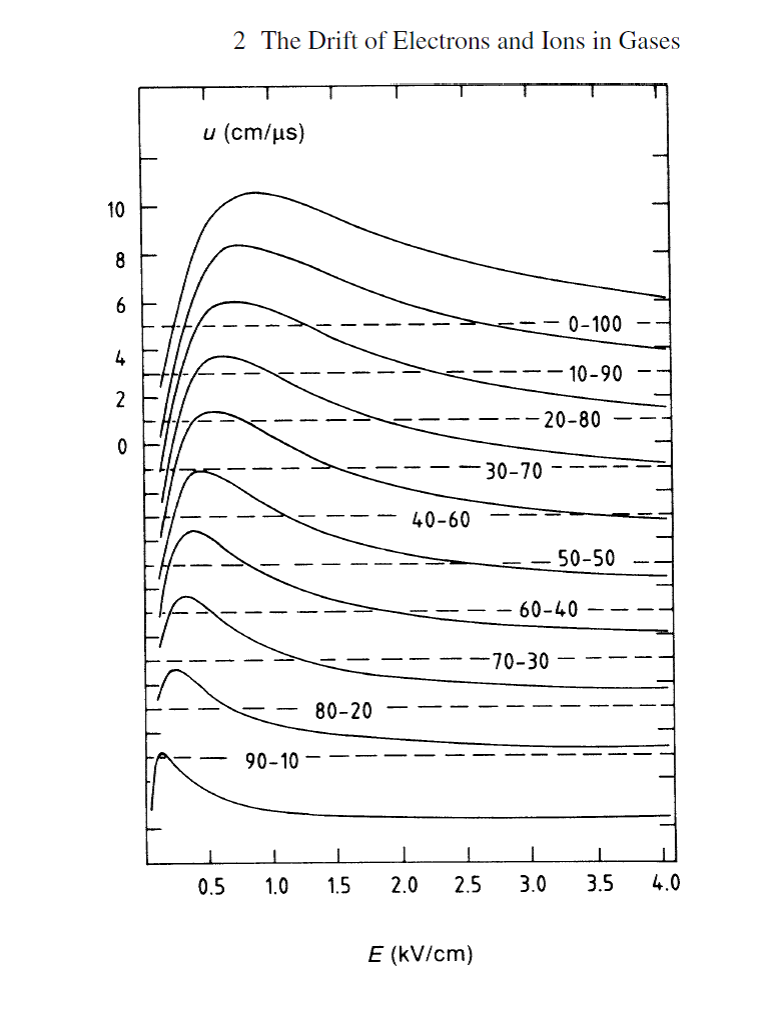
\includegraphics[width=8cm]{pics/drift_electrons.png}
    \caption{The drift velocity $u$ is plotted against the electric field strength for different argon-methane gas mixtures. This figure, based on measurements from Jean-Marie et al. [JEA 77], was taken from \cite{DriftChamberBook}, figure 2.17.}
    \label{fig:drift_electrons}
\end{figure}

\section{Gas Amplification}

If the accelerating electric field is strong enough, the electrons can gain enough energy between two collisions to ionize a gas atom. The new free electrons get accelerated themselves to the point where they can ionize a gas atom and the total number of free electrons increases rapidly in a snowballing effect. This "electron avalanche" can the be measured at the anode as a peak signal. This peak signal depends on the gas mixture and the applied electric field.

If the multiplication of electrons due to gas amplification occurs, the increase of the number of electrons per path $ds$ is given by
\begin{equation}
	dN = N\alpha ds
\label{multiplication}
\end{equation}
where $N$ is the number of electrons in the electron avalanche and $\alpha$ is the so-called first Townsend coefficient, determined by the properties of the gas as well as the local electric field. In particular, one can show that it depends on the electric field $E$ and the gas density $\rho$.
	
For our purposes, it is enough to directly integrate (\ref{multiplication}) and change the integration variable to be the electric field, i.e.
\begin{equation}
	N/N_0 = \text{exp} \int^{r_2}_{s_{\min}}\alpha(s)ds = \text{exp} \int^{E(r_2)}_{E_{\min}} \frac{\alpha(E)}{dE/ds}dE
    \label{basic_integral}
\end{equation}
Let us look at the different quantities in this equation: $r_2$ is the radius of the wire, while $s_{\text{min}}$ is the distance from the center of the wire to the point where the avalanche starts to form. $N$ is the number of electrons in the avalanche arriving at the wire, while $N_0$ is the number of electrons at the start of the avalanche. In particular, $N/N_0$ is the total increase of the signal due to the amplification. It is called the \emph{gain} and is denoted by $G$.
	
$E_{\text{min}}$ is the electric field at the starting point of the avalanche. However, we can also think of it as the minimal field strength needed to start an avalanche, which indicates that $E_{\text{min}}$ is a constant.
	
To simplify equation (\ref{basic_integral}), we make the assumption that the avalanche starts to develop only near the wires, where the field strength is strongest. This is motivated by the fact that, if the radius $r_2$ of the wire is small compared to the distance $r_1$ to the other electrode, we can assume that the field near the anode wire is given by the formula for a cylindrical geometry:	
\begin{equation}
	E(r) = \frac{1}{r}\frac{V}{\ln(r_2/r_1)},
	\label{cylindrical_field}
\end{equation}
where $r$ is the distance to the anode wire and $V$ is the voltage applied between the electrodes, i.e. the voltage \emph{difference} between anode and cathode. Note that for $r$ small enough, very high electric fields can be achieved, as claimed. Making this assumption allows us to compute explicitly $dE/ds$:
\begin{equation}
dE/ds = -dE/dr = \frac{1}{r^2}\frac{V}{\ln(r_2/r_1)} = \frac{\ln(r_2/r_1)}{V}E^2
\end{equation}
(note that the path goes into the opposite direction of $r$).
		
Furthermore, we use the Diethorn approximation which tells us that near the wire the Townsend coefficient is proportional to the electric field:
$$\alpha = \beta E,$$
where $\beta$ is some constant. Note that this approximation has been determined experimentally, and is valid in particular for noble gases such as the Argon that is in the drift chamber.
	
Inserting this expression into equation (\ref{basic_integral}) together with the expression for $dE/ds$ allows us to express the gain $G$ as follows:
\begin{equation}
	G = \text{exp }\left[\frac{\beta V}{\ln(r_2/r_1)} \int^{E(r_2)}_{E_{\min}}\frac{1}{E}dE \right] = \text{exp } \left[\frac{\beta V}{\ln(r_2/r_1)} \ln\left(\frac{E(r_2)}{E_{\min}}\right)\right].
\end{equation}
Inserting again (\ref{cylindrical_field}) for $E(r_2)$ and $V$, and using the Diethorn approximation $\alpha(r_2) = \beta E(r_2)$ to get rid of the $\beta$ we finally obtain:
\begin{equation}
\begin{split}
	G &= \text{exp }\left[\alpha(r_2)r_2\ln\left(\frac{V}{r_2\ln(r_2/r_1)E_{\min}}\right)\right]\\
	& = Ae^{r_2\alpha(r_2)\ln{V}},
\end{split}
\end{equation}
where $A$ is some constant that collects all other ones.
	
Now, in our case, we cannot directly measure the number of electrons reaching the wire. We can however measure the voltage difference that they induce when arriving on the anode, manifesting as a peak of height $P$. It is not hard to see that this voltage difference is proportional to the gain, i.e.
	
\begin{equation}
	P \propto e^{r_2\alpha(r_2)\ln{V}}.
\end{equation}

Thus the peak amplitude increases with increasing voltage. However this increase does not go on forever. If the charge of the avalanche is high enough to affect the electric field, the resulting signal is no longer proportional to the originally released charge.

Furthermore, if the voltage gets too high, electric discharges start to occur, where permanent gas discharges take place and a very high current flows. The equipment can be damaged in this process. 

This derivation followed closely \cite{DriftChamberBook}, in particular chapter 4.4.

\section{Cosmic Radiation}

Particles, in particular protons, coming from the universe and from the Sun constantly impact the Earth. The energy of these particles ranges from $10^9$ up to $10^{20}$ \SI{}{\giga\electronvolt}. The particles lose their energy by colliding with atoms in the upper atmosphere. In this process they create jets of new particles. Many of these secondary particles collide with gas atoms themselves and only a small fraction reaches the surface of the Earth.

 In the midst of these secondary particles there are also pions, which decay into muons and neutrinos after only a short amount of time. The neutral neutrinos only interact via the weak force and are practically undetectable. The charged muons lose energy due to ionization, but have cross sections for inelastic collisions with air atoms which are much smaller than the ones for the strongly interacting protons.

On the Earth's surface the cosmic radiation then consists mostly out of muons.

\section{Measurement Setup}

The mechanism consists of the actual drift chamber, the trigger, the electronics and a computer for data collection. Figure~\ref{fig:schema} shows a logic diagram of the setup. 

\begin{figure}[!h]
\includegraphics[width=13cm]{pics/Schema.jpg}
\centering
\caption{Logic diagram of the main parts of the measurement setup.}
\label{fig:schema}
\end{figure}

Figures~\ref{fig:NIM_crate} through \ref{fig:distributor} show the physical view of some of the elements in Figure~\ref{fig:schema}. It contains both the trigger logic units and power supplies. The units in Figure~\ref{fig:NIM_crate} are, from left to right:
\begin{itemize}
\item Lower voltage power supply for the amplifiers of the photomultipliers (PMTs)
\item Discriminator
\item Coincidence unit
\item Counter (counts the number of NIM signals)
\item Level converter (NIM to TTL)
\item High voltage power supply for cathode
\item High voltage power supply for anode (positive voltage)
\item High voltage power supply for field wires
\item Counter (counts the number of TTL signals)
\item Delay unit
\end{itemize}

\subsection{Trigger formation}
The trigger signal is formed in the following way: The muons crossing the scintillators produce photons in the scintillator. The photons are converted into an electrical pulse and further multiplied by the PMTs, and then fed into the discriminator. The discriminator analyzes the signal and if the amplitude of the signal crosses the set threshold, it outputs a square NIM pulse. The NIM pulses from each discriminator are then fed into the coincidence unit. This unit, when both inputs are set to AND mode, analyzes whether or not the input pulses overlap in time.
If they do, it outputs another NIM pulse, which in turn is fed into a first counter and at the same time into a TTL converter. The TTL pulse is then fed into a second counter. Each of the counters counts the pulses fed into it differently. The TTL pulse is then delayed by a delay unit, before going into the trigger input of the 1$^{st}$ DRS4 board.

When the trigger signal arrives there it gives the board a command to output the anode signals that are at the moment on the inputs of the DRS4 board to the computer. If the SAVE mode is activated, the inputs can be saved on the hard drive.

In parallel, another trigger output is fed into an external an oscilloscope, where one can observe the signals of the scintillators before and after they pass through the coincidence unit. You are strongly encouraged to explore the setup by yourself by tracing the cables. Understanding the trigger system is an important part of the experiment. 

\begin{figure}[!h]
\includegraphics[width=13cm]{pics/NIM_crate.JPG}
\centering
\caption{NIM crate with the main logic and power supplies.}
\label{fig:NIM_crate}
\end{figure}

Figures~\ref{fig:power_supply_front} and \ref{fig:distributor} show the front and back of the high voltage power supply of the scintillators. Note that the operation voltage of each scintillator differs slightly. The output of the high voltage power supply is fed into the 1st input of the high voltage distributor (Fig.~\ref{fig:distributor}), and the 1st and 2nd outputs of the distributor are then supplied individually to the scintillators. Each output can be regulated individually by a corresponding knob on the front panel of the distributor.

IMPORTANT: The power supply requires a few seconds to warm up before the high voltage can be switched ON. After turning on the power supply wait until the yellow/white indicator light is ON before flipping the high voltage switch to ON.

\begin{figure}
	\centering
		\begin{subfigure}[b]{0.8\textwidth}
				\includegraphics[width=1\linewidth]{pics/power_supply_distributor_front.JPG}
				\caption{}
				\label{fig:power_supply_front}
		\end{subfigure}
		\begin{subfigure}[b]{0.8\textwidth}
			\includegraphics[width=1\linewidth]{pics/distributor_back.JPG}
			\caption{}
			\label{fig:distributor}
		\end{subfigure}
\caption{The front (a)  and back (b) of the high voltage power supply and high voltage distributor for the scintillators.}
\end{figure}



\subsection{Drift Chamber}
\label{measurementsetupdriftchamber}

The electric field inside our drift chamber is generated by two parallel electrodes, which have a distance of \SI{94.3}{\milli\meter}. To have a homogeneous electric field inside the drift chamber, the potential also has to increase linearly from the cathode to the anode at the edge of the drift chamber. This is approximately achieved with 9 electrodes, which are placed parallel to each other in a distance of \SI{1}{\centi\meter} and enclose the drift chamber. Their potentials are linearly graduated with a bleeder chain. The resulting electric field looks similarly to the electric field in Figure~\ref{fig:potential}.

\begin{figure}[h]
\includegraphics[width=13cm]{pics/Potential}
\centering
\caption{Electric field lines and equipotential lines inside the drift chamber. The electrons drift from left to right, where the signal wires are.}
\label{fig:potential}
\end{figure}
 
Figure~\ref{fig:drift_chamber_cross_section} shows a CAD cross section of the drift chamber. The anode wires, which produce the gas amplification, are placed \SI{4.2}{\milli\meter} in front of the ground plate. The sensitive region in which the particles can be detected is between those wires and the cathode and has a length of \SI{94.3}{\milli\meter}.

\begin{figure}[!h]
	\includegraphics[width=13cm]{pics/Driftkammer_Schnittbild.jpg}
	\centering
	\caption{CAD cross section of the drift chamber. All the distances shown are correct. The chamber has 8 anode wires (shown as black dots on the left side of the picture). On each side of the anode wires the field wires (empty circles) are located equidistantly from each anode neighboring anode wire. The cathode plate is \SI{94.3}{\milli\meter} right of the anode wires. About \SI{4.2}{\milli\meter} to the left of the anode wires the ground plate is located. On top and bottom of the sensitive region the field plates are separated from each other with roughly equal distances.}
	\label{fig:drift_chamber_cross_section}
\end{figure}

The 8 anode wires are arranged parallel to each other and have a distance of \SI{10}{\milli\meter} between each other. Their radius is only \SI{25}{\micro\meter}, so they can produce the needed high electric field strengths for the gas amplification. Between the anode wires there are field wires that make the electric field more even. These field wires have an own voltage supply, which can be left at zero. 

The anode wires are connected to a an amplifier powered by a low voltage power supply, which amplifies the signal coming from the wire even further. This amplifier is mounted inside the drift chamber, at the end of each anode wire. The low voltage power supply is connected to the amplifier by three jacks at the front of the chamber and has to be turned on in order to detect the signals on the anode wires. 

The drift chamber is mounted in such a way that the wires are horizontal and the plane of the wires is vertical. The drift direction for the electrons is thus horizontal. A particle which travels vertically through the drift chamber will therefore induce a signal in all wires. Figure~\ref{fig:CAD} shows the interior of the drift chamber with the electrodes and the signal wires. 

\begin{figure}[h]
\includegraphics[width=13cm]{pics/Driftkammer_Ansicht_5.png}
\centering
\caption{A schema of the drift chamber. One can observe the anode wires (the field wires between the anode wires are not shown), the electrodes which make a more homogeneous field and the cathode and ground plate.}
\label{fig:CAD}
\end{figure}

\subsection{The DRS4 unit}
To process the incoming data from the signal wires, the wires are connected to DRS4 boards. These DRS4 boards were designed at the Paul Scherrer Institute and are capable of digitizing 4 channels each. Two boards are linked together to process all 8 channels. The DRS4 boards work like a digital oscilloscope. For details on the operation of the DRS4 boards please refer to the DRS4 manual \cite{DRS4_manual}.

The DRS4 unit comes with a computer program called drsosc located in \verb|~/Desktop/drs-5.0.6/|. A softlink to the executable is put in the home directory. The program can be started from the command line as follows: 

\begin{lstlisting}[language=bash]
$ ./drsosc
\end{lstlisting}

 It opens a GUI that emulates an oscilloscope interface and can display all 8 channels. The boards have a port for an external trigger which can be connected to the trigger logic. The trigger output of the first board is connected to the second board, so both boards receive the trigger at approximately the same time.

\section{Measurements}
The main goal of this experiment is to familiarize oneself with the operation of a small drift chamber and observe the tracks of cosmic muons passing through it. Additionally, you will develop your own data analysis technique using a provided data conversion program as a starter. You are advised to perform the following measurements. Start with finding the working point of the scintillators. Then study the dependence of the gas amplification with respect to the anode voltage, followed by the study of the dependence of the electron drift velocity for varying cathode voltages. Finally, observe a few events for which you can plot the muon traces. The following sections will give you some hints on how to perform the measurements. Overall you are encouraged to develop your own methods to measure the parameters mentioned above. However, if your methods deviate from the suggested, substantiate them by solid physical arguments. 

\subsection{Saving and analyzing data}
Save your data in binary format. It is important to add a \verb|.dat| to the file name, otherwise the analysis code which will convert your binary format into either a ROOT file or a text file will not work. The codes and more information about them are in the appendix \ref{sec:decode}. The ROOT version can be found in the directory \verb|~/Software/driftchamber/code/|. Please NOTE that the extensions to the analysis codes should be written by you! 

\subsection{Basic setting}
Here we summarize some basic settings that will result in workable signals and that you can use as a starting point to see if everything works. See figures \ref{fig:oscilloscope}, \ref{fig:DRS_oscilloscope_settings}, \ref{fig:DRS_oscilloscope_settings_configuration}, \ref{fig:field_plate_generator} and \ref{fig:delay_unit} for details about the settings of the external oscilloscope and the DRS4 software.

Here are the different voltages that have to be set:

\begin{itemize}
    \item Anode voltage: \SI{3000}{\volt}
    \item Cathode voltage : \SI{4000}{\volt}
    \item Field wires current: \SI{0}{A}
    \item Delay : About \SI{1.5}{\micro\second} (see figure \ref{fig:delay_unit}; try not to change it)
\end{itemize}

Both scintillators also have to be set on AND, and the DRS4 software has to be set to trigger on the external signal.

For the external oscilloscope, the inputs were set as follows:
\begin{itemize}
    \item Channel 1: CH4, i.e. first scintillator
    \item Channel 2: CH3, i.e. second scintillator
    \item Channel 3: CH1, i.e. first discriminator
    \item Channel 4: CH2, i.e. second discriminator
    \item External Trigger: Coincidence
\end{itemize}

\begin{figure}[H]
    \centering
    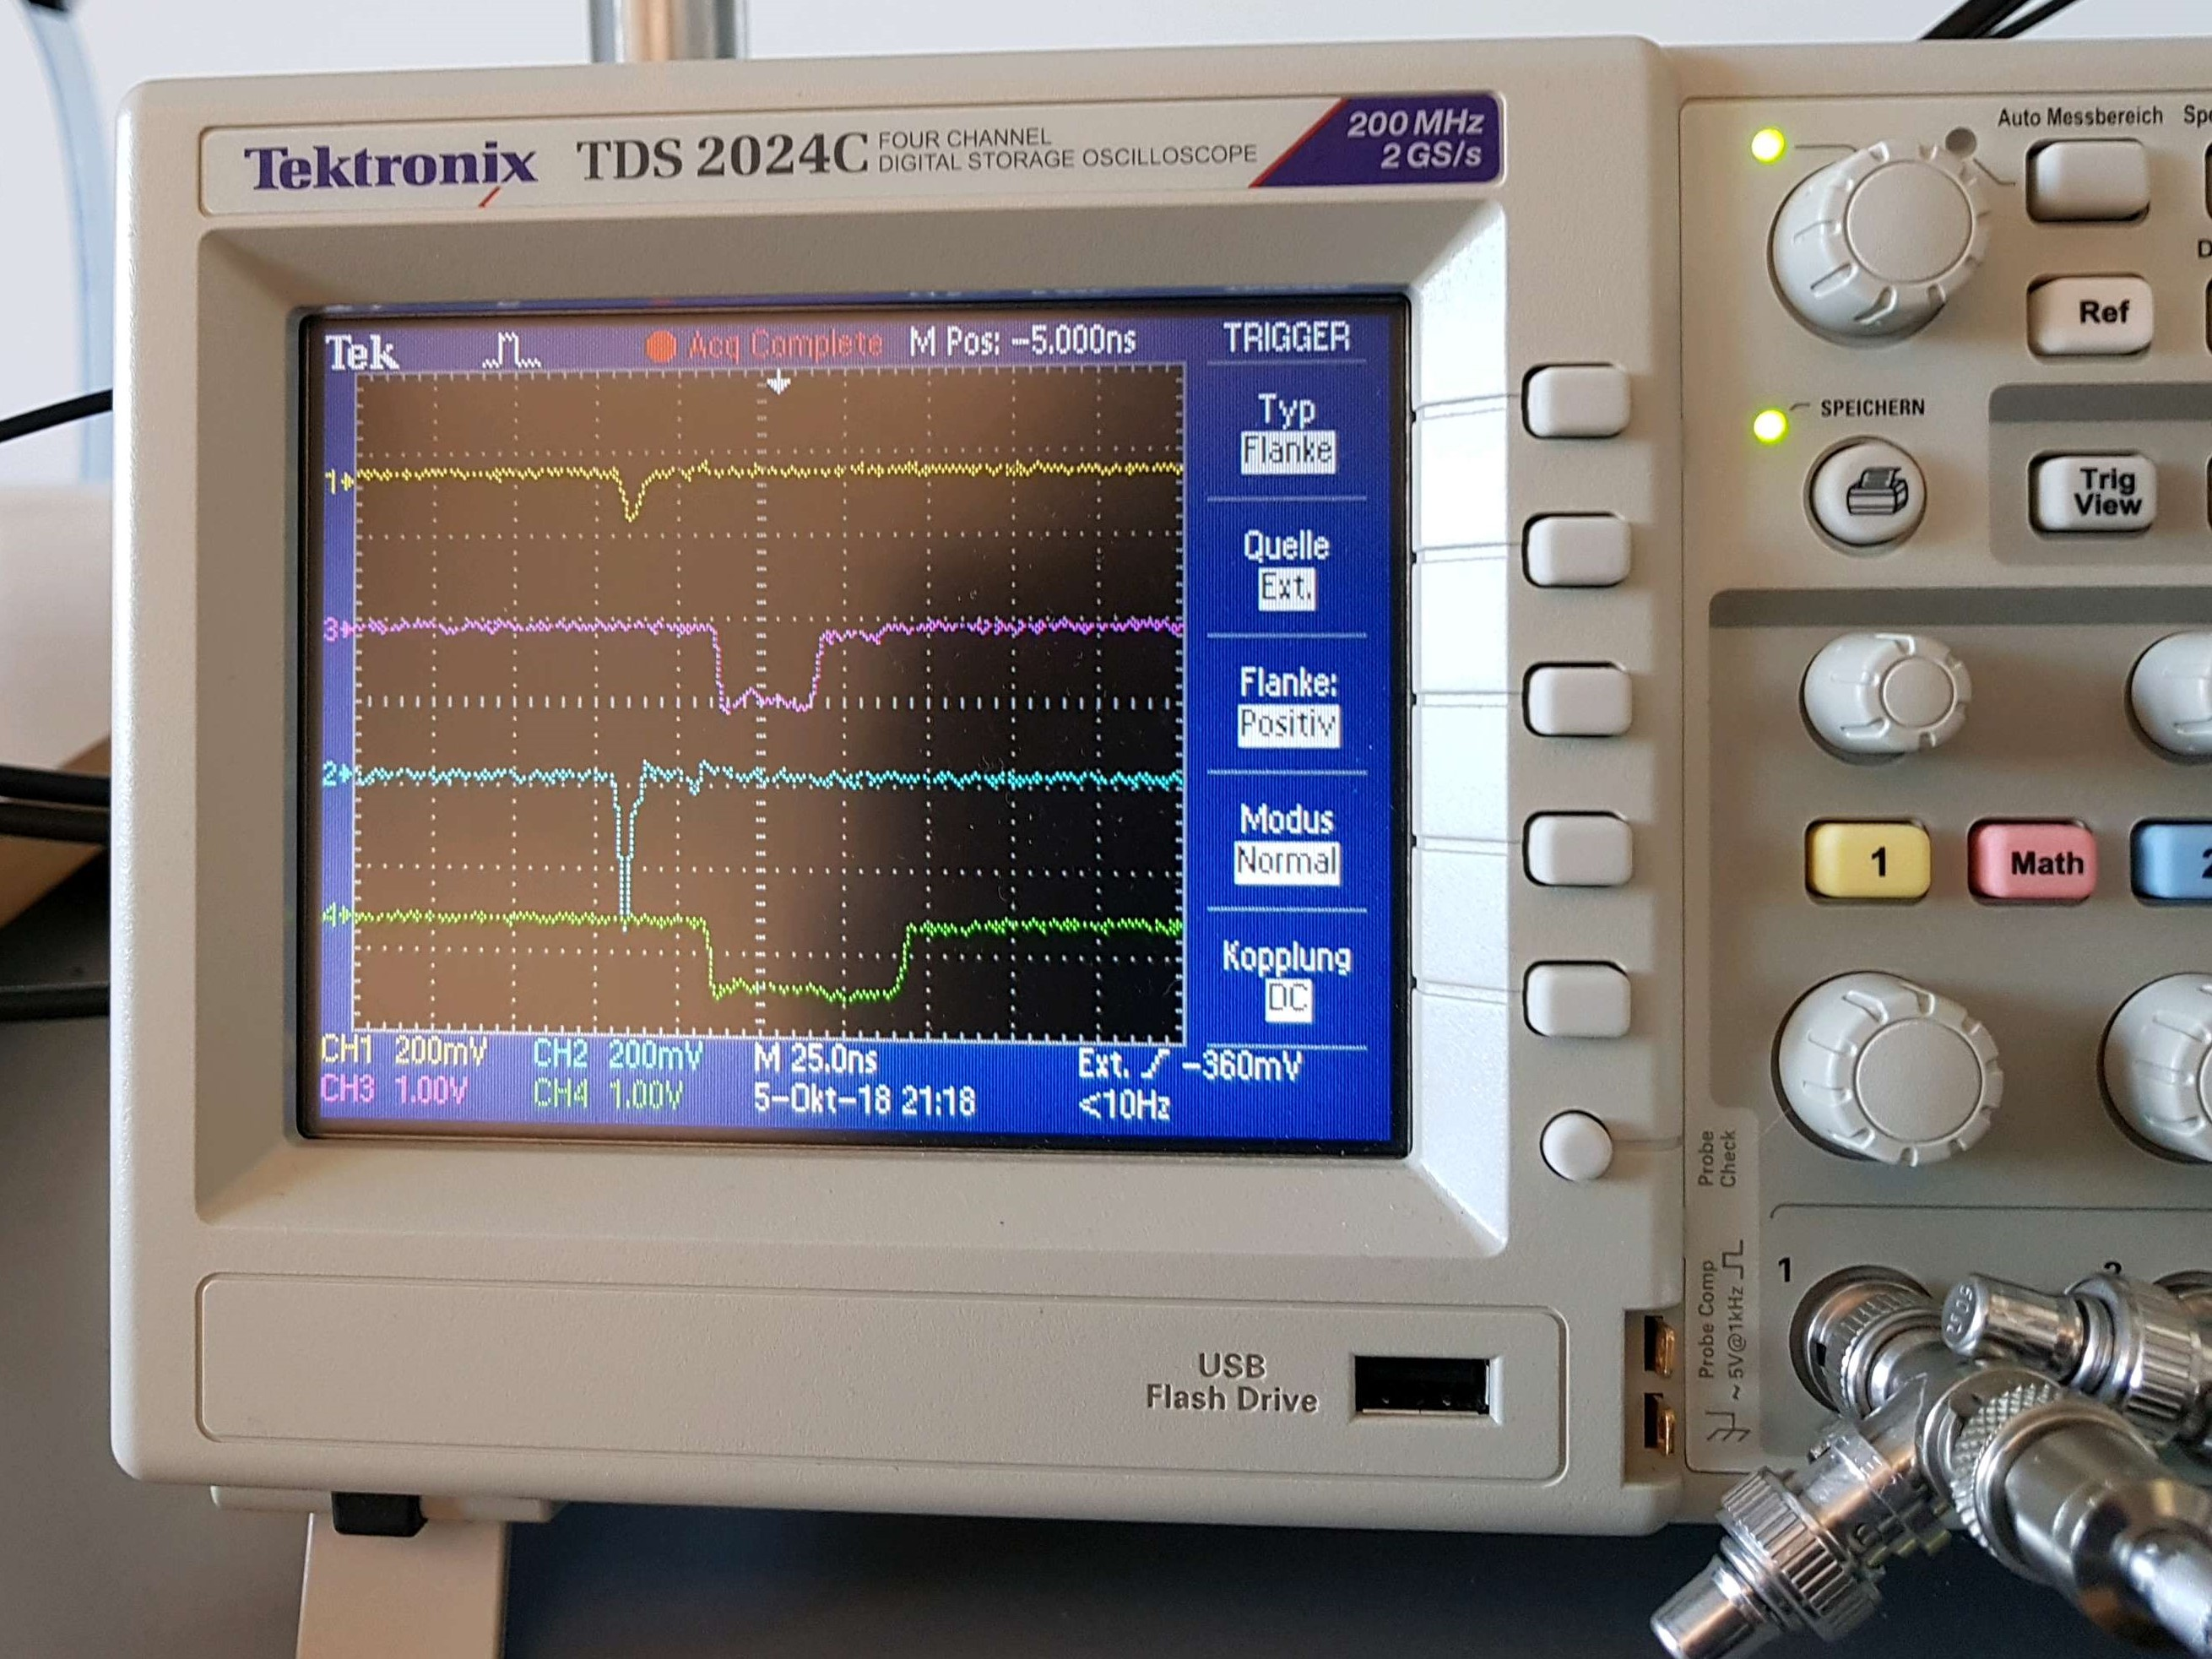
\includegraphics[width = 13cm]{pics/oscilloscope.jpg}
    \caption{\small The main adjustment for the oscilloscope is shown. The yellow and the blue signal are the signals of the scintillators and the the purple and the green signals are from the discriminators. The vertical and horizontal scaling as well as the trigger level can be seen on the bottom of the screen.}
    \label{fig:oscilloscope}
\end{figure}
\begin{figure}[H]
    \centering
    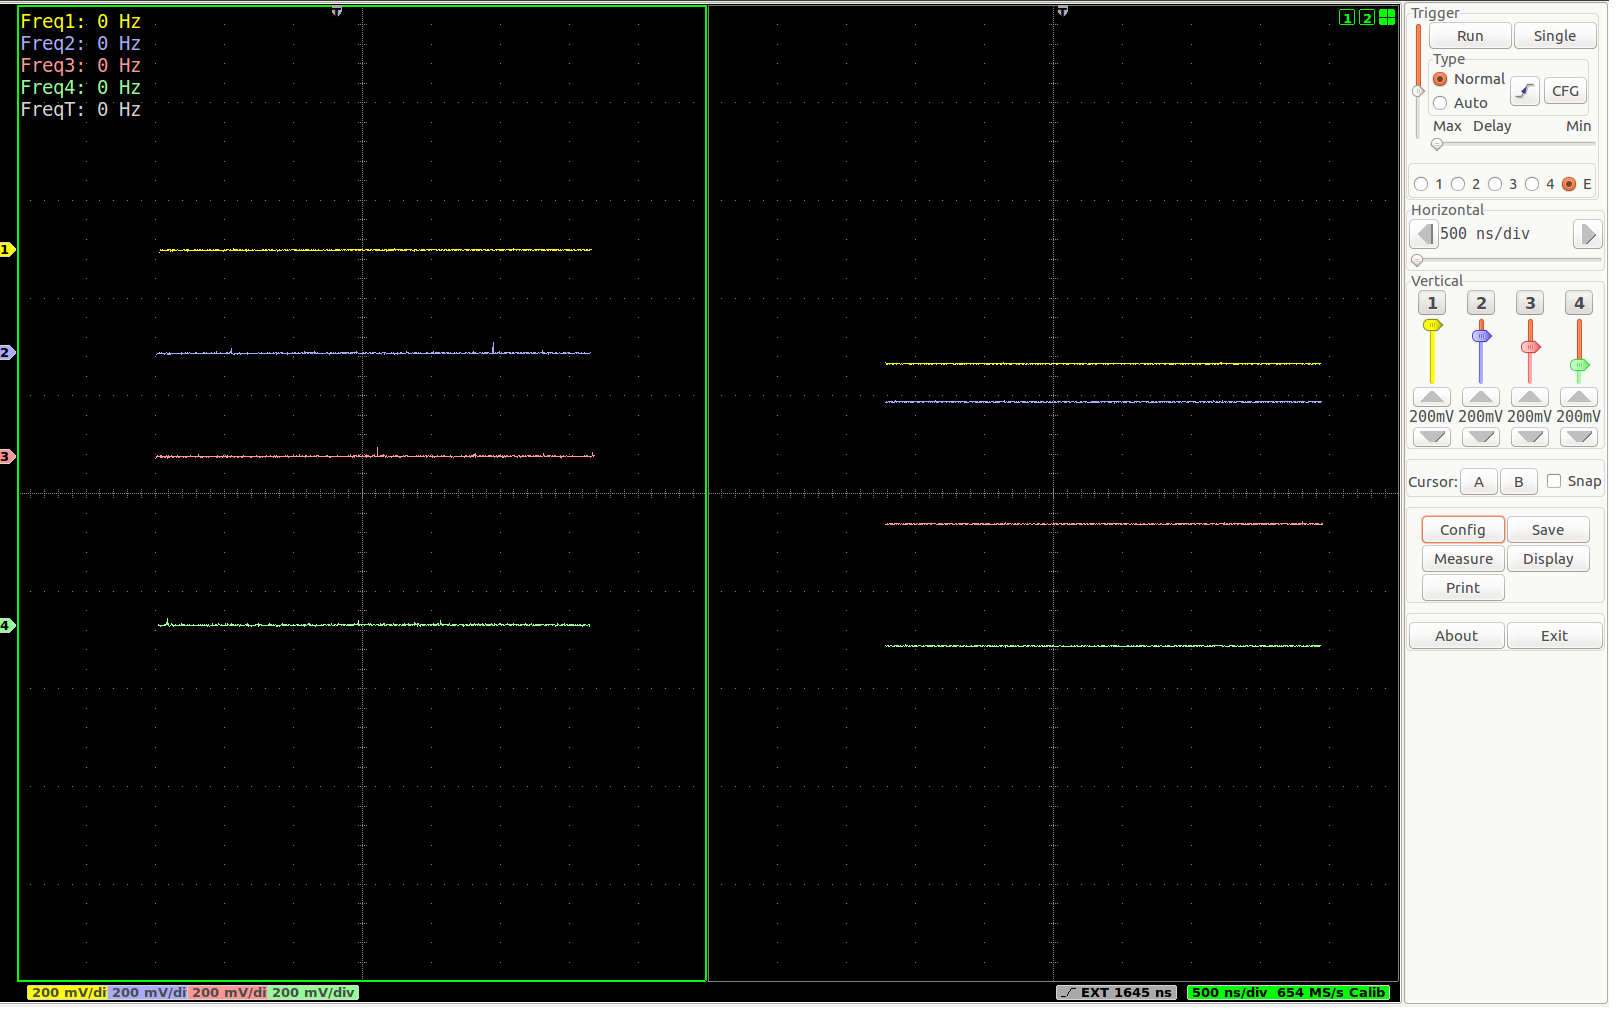
\includegraphics[width = 9cm]{pics/DRS_oscilloscope_settings.png}
    \caption{\small Main screen of the DRS4 software GUI. The settings for the vertical and horizontal scaling as well as the trigger time (corresponds to the origin in the graphs) can be seen on the bottom of the window. On the top right corner, the trigger can be set to be one of the 4 first channels, or the external trigger logic. For the basic setting, set the trigger to external. See also figures \ref{fig:DRS_oscilloscope_settings_details_top_right} and \ref{fig:DRS_oscilloscope_settings_details_scaling} for greater details}
    \label{fig:DRS_oscilloscope_settings}
\end{figure}
\begin{figure}[H]
    \centering
    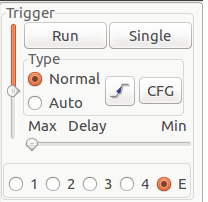
\includegraphics[width = 3cm]{pics/DRS_oscilloscope_settings_details_top_right.png}
    \caption{\small Top right corner of the DRS4 GUI, where the trigger can be set.}
    \label{fig:DRS_oscilloscope_settings_details_top_right}
\end{figure}
\begin{figure}[H]
    \centering
    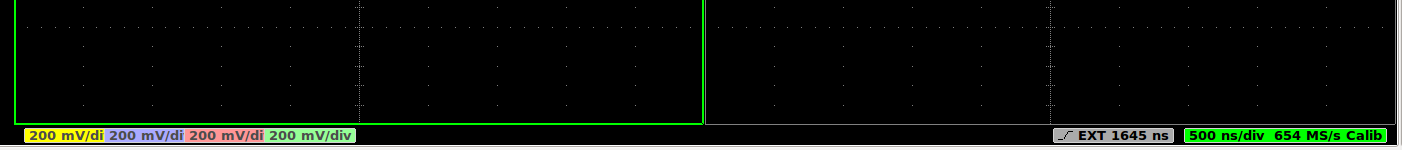
\includegraphics[width = 11cm]{pics/DRS_oscilloscope_settings_details_scaling.png}
    \caption{\small Bottom of the DRS4 GUI, where the scaling settings can be seen.}
    \label{fig:DRS_oscilloscope_settings_details_scaling}
\end{figure}
\begin{figure}[H]
    \centering
    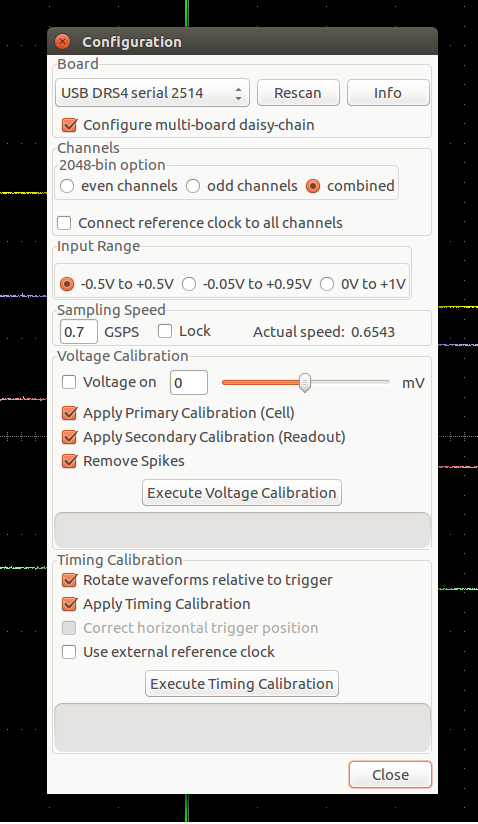
\includegraphics[width = 8cm]{pics/DRS_oscilloscope_settings_configuration.png}
    \caption{\small Details of the configuration of the DRS4 oscilloscope. The default parameters should be fine for all measurements, and should thus ideally not be changed.}
    \label{fig:DRS_oscilloscope_settings_configuration}
\end{figure}
\begin{figure}[H]
    \centering
    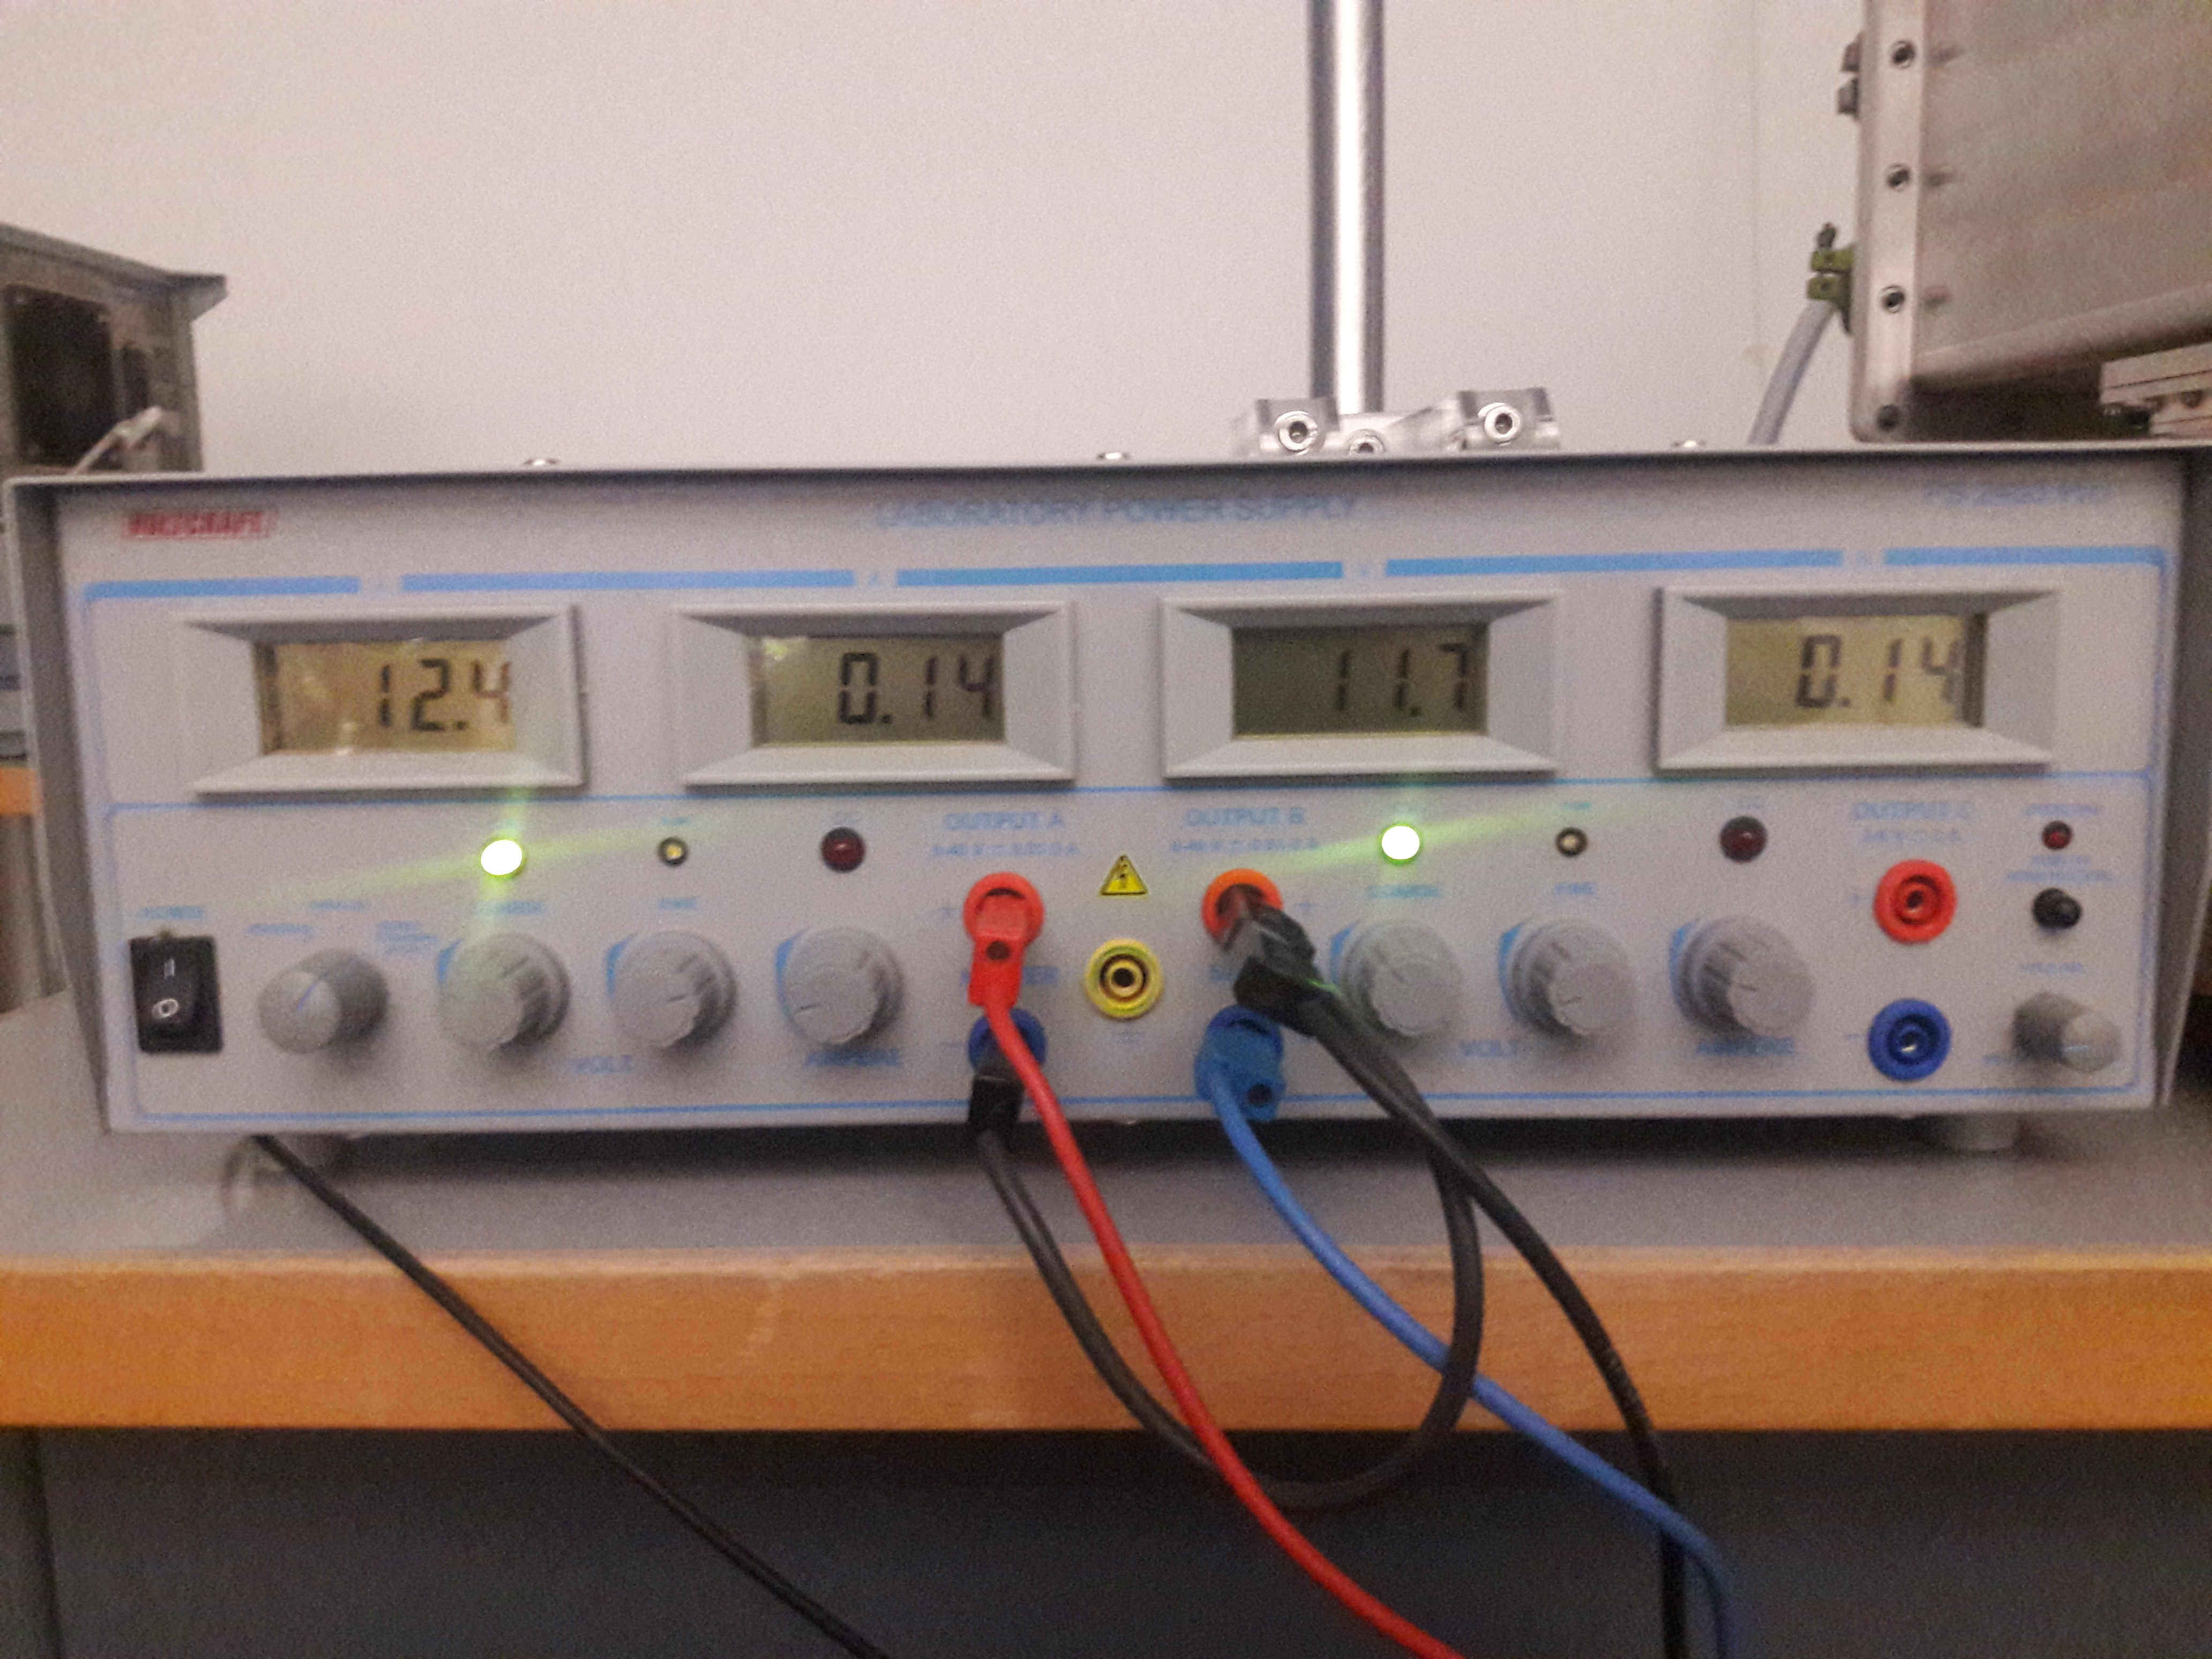
\includegraphics[width = 9cm]{pics/field_plate_generator.jpg}
    \caption{\small Typical settings for the voltage applied to the field plate electrodes. The default values should be fine for all measurements, and should thus ideally not be changed.}
    \label{fig:field_plate_generator}
\end{figure}
\begin{figure}[H]
    \centering
    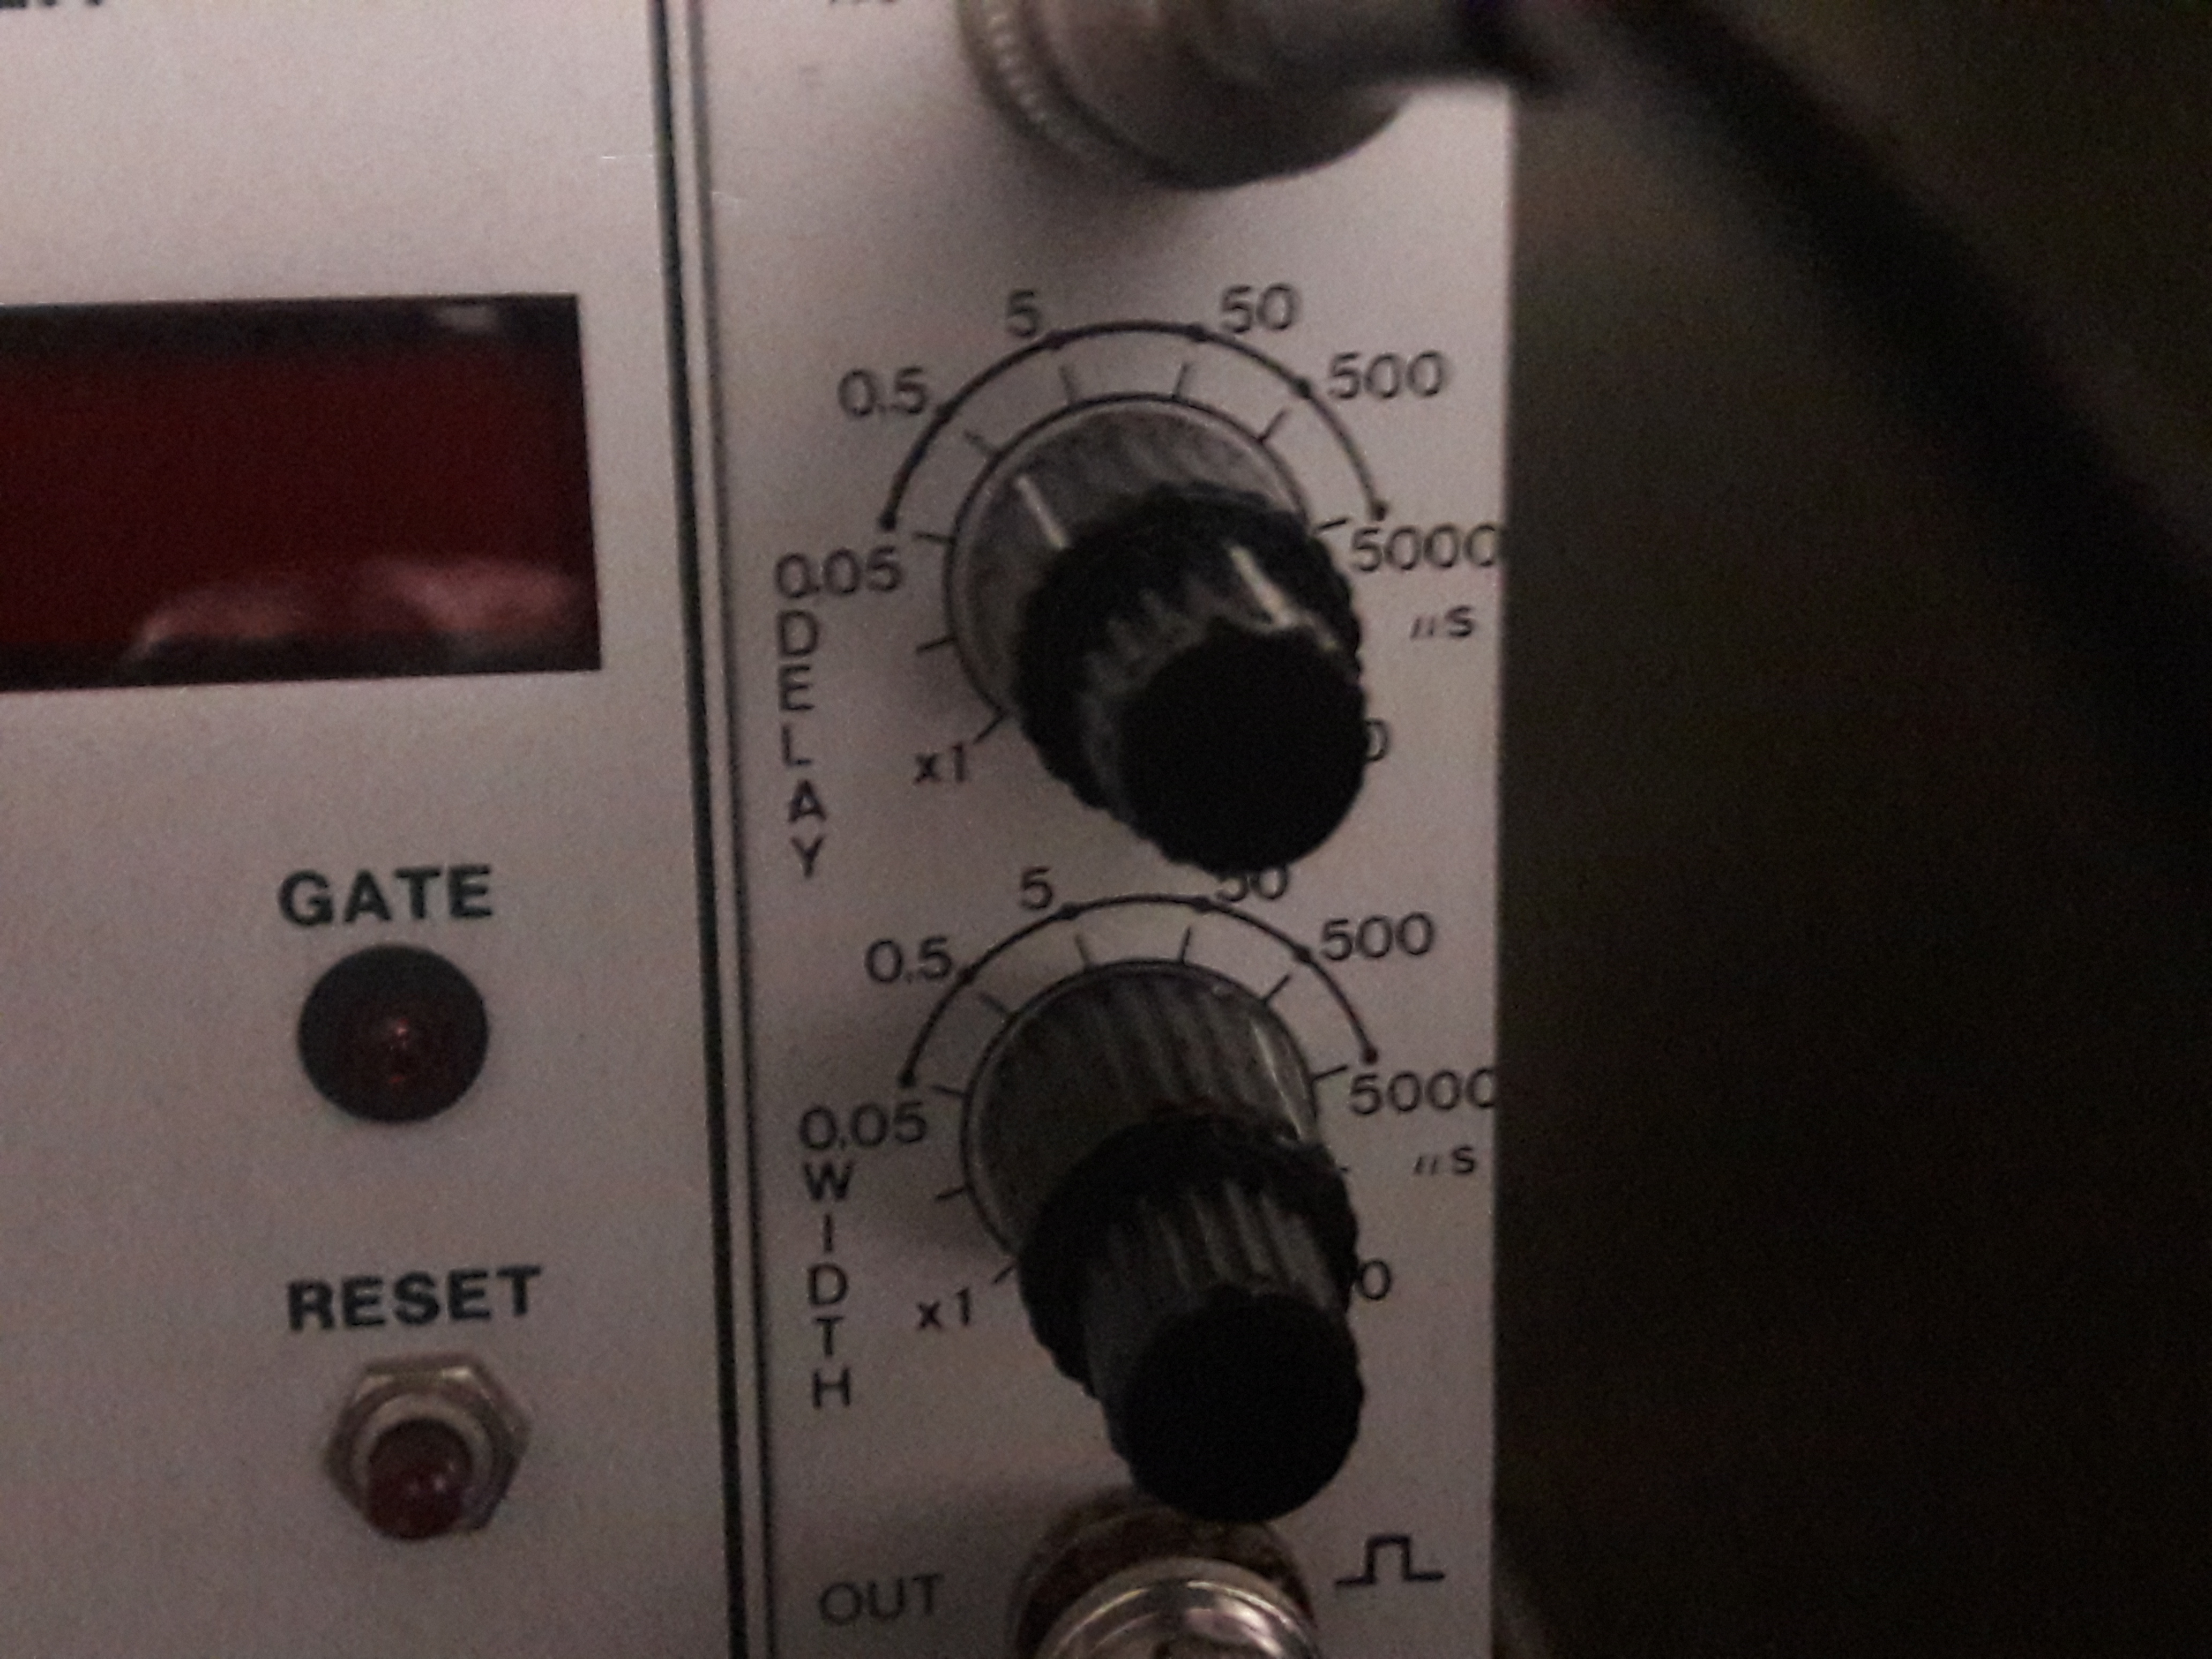
\includegraphics[width = 9cm]{pics/delay_unit.jpg}
    \caption{\small Typical settings for the delay and width of the signal produced by the delay unit. The default values should be fine for all measurements, and should thus ideally not be changed.}
    \label{fig:delay_unit}
\end{figure}

\subsection{Finding the working point of the scintillators}
To get a good trigger signal you first have to find the working point of the two scintillators. For any given discriminator threshold the scintillator has a specific voltage, where all incoming signals get detected, but the voltage is not high enough to detect too much background noise. This manifests itself as a plateau in the counts per second around this working point. You apply a voltage of about \SI{2}{\kilo\volt} on the scintillators and put one of them to AND on the coincidence unit. Then you can regulate the threshold so that there are a few counts per second. The threshold voltage can be measured with the external voltmeter. It is strongly recommended to leave the threshold as it is and only change the anode voltage. Now you have to count the triggered signals and calculate the number of counts per second for different applied voltages from around \SI{1.9}{\kilo\volt} to \SI{2.1}{\kilo\volt}. Plot the counts per second against the voltage and you will see a plateau. The working point of the scintillator is the highest voltage of the plateau. Repeat the measurement for the second scintillator. The working points of the scintillators do not have to be at the same voltage, but double check if the plateaus have similar number of counts per second.

\subsection{Purifying the gas}
The experiment is performed at an atmospheric pressure. The gas inside the chamber is a mixture of argon and methane (50:50). It is supplied from the pressurized gas cylinder marked (A) on Figure~\ref{fig:gas}. The chamber is also connected to a pressure pump (D), which can evacuate the chamber. In order to evacuate the chamber the valve at the chamber to the pump (B) and the valve at the pump itself should both be opened. While the valve to the gas cylinder (C) should be closed. The filling of the chamber is performed by closing the valves (B) and (D) and opening valves (A) and (C). Before starting the experiment it is wise to empty the chamber and fill it up again several times, to make sure the gas inside the chamber is pure enough. The pressure inside the chamber should be at or slightly above \SI{1}{\bar} in the end.

IMPORTANT: When you finish purifying the gas inside the chamber make sure that the valve (A) on the gas cylinder is closed.

\begin{figure}[!h]
	\includegraphics[width=12cm]{pics/valve}
	\centering
	\caption{To evacuate the chamber turn on the pump under the table and open valve (D) and (B). Do open valve (B) gently, such that the pressure does not decrease too fast, otherwise it will start to smell. To stop evacuating first close valve (B) and then (D). To fill the chamber with gas, first open valve (A) and then gently open valve (C) until the desired pressure is achieved. Afterwards close valve (C) and (A).}
	\label{fig:gas}
\end{figure}

\subsection{Gas Amplification}
In the next part you want to find the optimum anode voltage that provides the maximum amplification while keeping the frequency of the sparking (electrostatic discharge) inside the chamber low. 

In order to have a high enough count rate, a \isotope[90]{Sr}-probe can be put on the window on top of the drift chamber. This isotope decays in a $\beta^-$-decay into \isotope[90]{Y}, which is also a $\beta^-$-emitter. The electrons from the $\beta^-$-decays have a wide energy spectrum up to a maximum energy of \SI{2.28}{\mega\electronvolt}. The scintillators and the metal walls of the drift chamber stop these low-energy electrons, which is why the source has to be placed on the window and the DRS4 board should be set to trigger on one of the channels.

% Then find the lowest anode voltage at which you can see triggered signals on the oscilloscope. Set the trigger as low as possible, but high enough that the noise does not trigger the oscilloscope. With the oscilloscope you can take the mean over several pulses. Then the average pulse amplitude can be read. It is important to set the threshold of the trigger as low as possible, because a trigger which is set too high can falsify the average signal amplitude.

Then you have to repeat the measurement for increasing anode voltages and plot the average pulse amplitude against the \emph{total} applied voltage. Be careful with increasing the voltage, because the actual voltage follows the adjusted value with some delay. Increase the voltage only in small steps and wait until it stabilizes. If you see a breakdown on the oscilloscope, immediately decrease the anode voltage. Figure~\ref{fig:breakdown} shows how a typical breakdown looks like on the oscilloscope. Do not increase the anode voltage over \SI{4}{\kilo\volt}. 

\begin{figure}[h]
\includegraphics[width=10cm]{pics/breakdown}
\centering
\caption{A picture of a typical display of an oscilloscope at the time of a breakdown. The anode voltage inside the drift chamber gets too high and electric discharges occur, which produce this signal. If a breakdown is visible or audible inside the chamber, the anode voltage has to be decreased immediately.}
\label{fig:breakdown}
\end{figure}

\subsection{Drift Velocity}
Now set the anode voltage to the optimal value, which was determined in the previous task. Because we now want to make a time measurement, the external trigger should be used. The scintillators must be placed above and below the drift chamber. The scintillators should be positioned exactly vertically above each other and the coincidence unit should be set to AND for both scintillators. In order to find the time an electron needs to travel from the cathode plate (\SI{94.3}{\milli\meter}) to the anode wire, the events with the earliest signals (muon passes next to the anode wire) and the latest signals (muon passes next to the cathode plate) should be observed. Note that because of the geometrical acceptance of the scintillator trigger, such events have very low probability (you are encouraged to estimate this probability). Therefore a significant amount of events ($\sim$1000) should be recorded.

 With the assumption of a constant velocity you can then derive the drift velocity. Repeat this measurement for several cathode voltages between \SI{500}{\volt} and \SI{4000}{\volt} to see how the drift velocity depends on the cathode voltage. The exact amount of points you need to choose will depend on your time and curiosity.

\subsection{Muon tracking}

Now you have all the needed data to reconstruct the track of the muons. You can either collect a small amount of data at you favourite settings or use a sample of the data from the drift velocity measurements. The drift velocity will help you to compute the distance at which the muon passed the signal wire. Then using the vertical positions of the wires plot the trajectories.

\bibliographystyle{unsrt}
\bibliography{driftchamber_references}

\pagebreak

\appendix
\section{Sample Analysis Code:}\label{sec:decode}
In order to read the output of the DRS4 software, you first need to translate the binary file into readable format. To do so, you can use one of the two following codes:

The first one can be called as
\begin{lstlisting}[language=bash]
  python decode.py filename.dat
\end{lstlisting}
(note that the file name has to end with .dat) and transforms the file into a ROOT file. ROOT is a programming/data-base language used primarily at CERN. The ROOT website is located here:
\url{https://root.cern.ch/}

If you plan to use python and ROOT together, it is strongly recommended to install ROOT on a Linux system. You can find instructions on how to do so on the internet (they may change depending on your version of Linux).

The second code takes the same input as the first one and outputs a directory with the transformed data. It can be called as
\begin{lstlisting}[language=bash]
  python decode.py filename.dat
\end{lstlisting}
and yields a folder \verb|filename_Data| in which the data for each channel is written in separate files, for example \verb|filename_chn1_v|, \verb|filename_chn1_t| for the voltages and times of channel 1 respectively.

These files can then be opened and read using the numpy function.
\begin{lstlisting}[language=Python]
    voltages = loadtxt("filename_chn1_v")
\end{lstlisting}
This yields a 2-dimensional numpy array. In this case, voltages[0] are the voltages measured for the first measurement/event, and similarly for the time measurements.

As the root language can be somewhat long to learn, this second version provides a quick alternative for reading the data given by the DRS4. However, the output files are much bigger than they would be for the ROOT-version and take much more time to compile.

\subsection{ROOT Version}
The latest analysis code is located at:

\url{https://github.com/dmitryhits/driftchamber/blob/master/code/decode.py}
\lstinputlisting[language=Python]{decode.py}

\subsection{Text-like Version}
\lstinputlisting[language=Python]{decode_text.py}

\end{document}
